\documentclass[10pt]{beamer}
\usepackage{xeCJK}
\usepackage{listings}

\usetheme[
	sidebar, % 默认不显示包含幻灯片结构的边框。如设置sidebar选项,则参考AAU模板显示左边框
	footline,
	blue, % 主色调默认为红色,色调可以选择red和blue
%	wide, % 幻灯片的长宽比默认为4:3,如设置了wide选项则为16:9
	hideallsubsections, % 默认显示所有等级的标题。如设置了hideallsubsections,
	                    % 则不显示小节标题
	mathserif, % 默认公式字体是钝化的,如设置mathserif选项则采用正常的公式字体
	english, % 默认幻灯片环境为中文,如设置english选项则采用英文的章节和图表编号
	sectiontoc, % 设置sectiontoc选项则在每节(section)之前添加一个所有节的目录,
	            % 并标明本节在整个幻灯片中的位置,不建议和\part层级一同使用
]{SEUstyle}

\lstset{frame=shadowbox,
	language=[LaTeX]Tex,
	keywordstyle=\color{red}\bfseries,
	commentstyle=\color{gray}
}

\title[使用手册]{SEU Beamer模板使用手册}
\author[张舒韬]{张舒韬 \\ Shutao Zhang}
\institute[SEU KSE Lab]{东南大学\ 计算机科学与工程学院\ 知识工程实验室}

\begin{document}
	{\background
		\begin{frame}[plain,noframenumbering]
			\titlepage
		\end{frame}
	}
	
%	\part[简介]{SEU Beamer模板简介}
	
	\section{模板简介}
	\begin{frame}{SEU Beamer模板简介}
		\begin{itemize}
			\item<1-> SEU Beamer模板的设计和编写旨在提供一个东南大学专用的LaTeX幻灯片模板。
			\item<2-> SEU Beamer模板是在\alert{AAU的sidebar beamer模板}和\alert{西安电子科技大学的XDU beamer}模板上修改所得的。
		\end{itemize}
	\end{frame}

	\section[使用方法]{模板使用方法}
	
	\begin{frame}{模板使用方法}{模板结构}
		SEU Beamer模板的目录下包括以下文件:
		\begin{description}
			\item[beamerthemeSEUstyle.sty] 调用SEU Beamer模板的入口
			\item[beamerouterthemeSEUstyle.sty] SEU Beamer的外部主题,
				主要控制的是幻灯片顶部尾部的信息栏、边栏、图标、帧标题等一帧之外的格式
			\item[beamerinnerthemeSEUstyle.sty] SEU Beamer的内部主题,
				主要控制的是标题页,列表项目、定理环境、图表环境、脚注在一帧内的内容格式
			\item[beamercolorthemeSEUstyle.sty] SEU Beamer的色彩主题,控制各个部分的色彩
			\item[XDUtheme目录] 包含SEU Beamer中用到的图片资源,包括东南大学的logo
		\end{description}
	\end{frame}

	\begin{frame}{模板使用方法}{调用方法}
		\begin{itemize}
			\item 将目录SeuBeamerTheme下的所有文件复制到目标目录
			\item 在主文件的导言区添加以下代码:
				\lstinputlisting{demo_preamble.tex}
				其中options为相关参数选项
			
		\end{itemize}
	\end{frame}
	
	\begin{frame}{模板使用方法}{参数说明}\label{frame:args}
		命令\alert{usetheme}包含以下几个选项参数:
		\begin{description}
			\item[sidebar] 默认不显示包含幻灯片结构的边框。如设置该选项,则参考AAU模板显示左边框,包含所在部分(part)的目录
			\item[footline] 该选项设置正文下方信息栏的显示
			\item[blue] 主色调默认为红色,色调可以选择red和bule
			\item[wide] 幻灯片的长宽比默认为4:3,如设置了该选项则为16:9
			\item[hideallsubsections] 默认在目录中显示所有等级的标题。
				如设置了该,则不显示小节标题
			\item[mathserif] 默认公式字体是无衬线的,如设置该选项则采用正常的公式字体
			\item[english] 默认幻灯片环境为中文,如设置该选项则采用英文的章节和图表编号
			\item[sectiontoc] 设置该选项则在每节(section)之前添加一个所有节的目录,并标明本节在整个幻灯片中的位置,不建议和\alert{part}层级一同使用
		\end{description}
	\end{frame}

	\begin{frame}{模板使用方法}{首页和尾页}
		\begin{itemize}
			\item 幻灯片的首页和尾页采用background背景,并采用plain,noframenumbering选项
			\item 首页代码示范:
				\lstinputlisting{firstpage.tex}
			\item 尾页代码示范
				\lstinputlisting{lastpage.tex}
		\end{itemize}
	\end{frame}

%	\part[案例]{使用案例}
	
	\section{使用案例}
	\begin{frame}{使用案例}{左边框的显示}
		左边框的显示由sidebar选项控制,显示效果如下:
		\begin{figure}
			\centering
			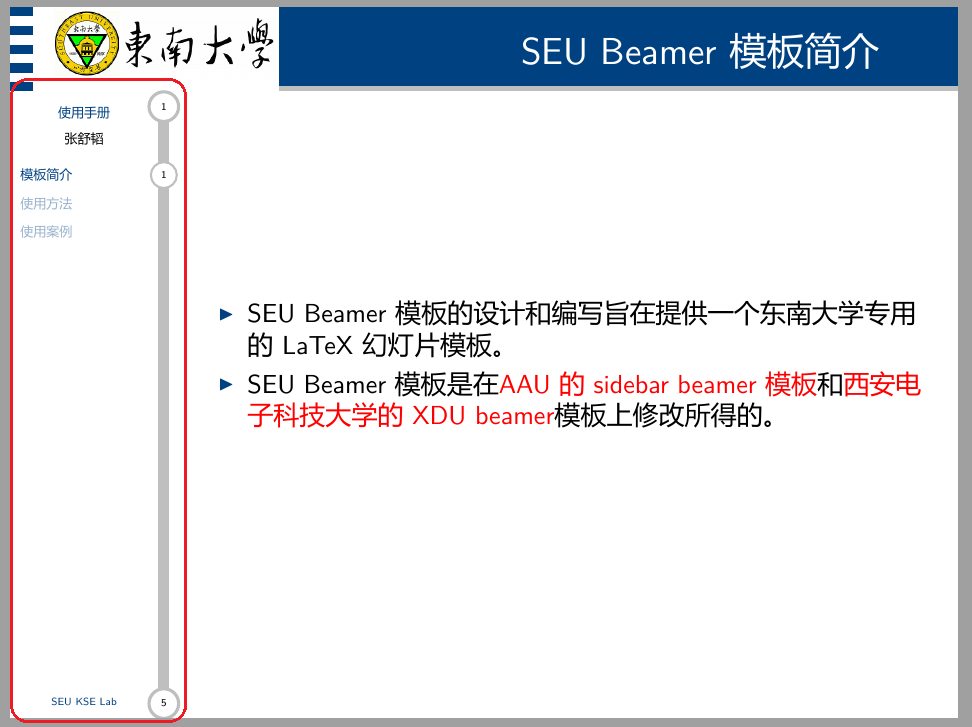
\includegraphics[width=0.7\linewidth]{pictures/sidebar}
			\caption{左边框在幻灯片中的显示}
			\label{fig:sidebar}
		\end{figure}
	\end{frame}

	\begin{frame}{使用案例}{章节目录的显示}
		每节之前的目录的显示由sectiontoc目录控制,显示效果如下:
		\begin{figure}
			\centering
			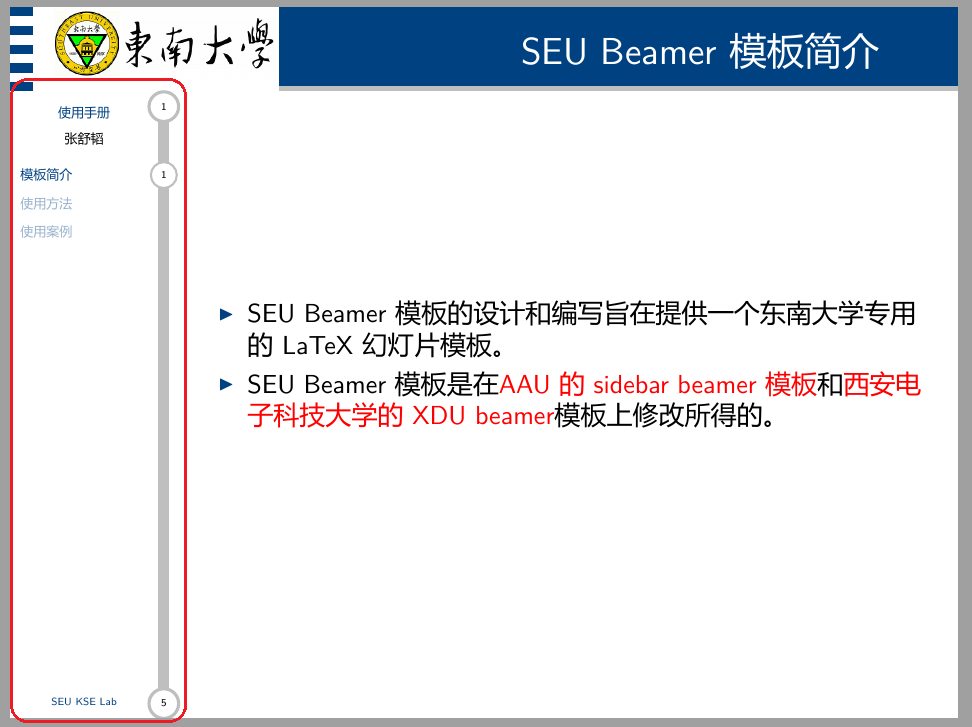
\includegraphics[width=0.7\linewidth]{pictures/sidebar}
			\caption{左边框在幻灯片中的显示}
			\label{fig:sidebar}
		\end{figure}
	\end{frame}
	
	{\background%末页致谢
		\begin{frame}[plain,noframenumbering]
			\finalpage{{\huge 感谢观看!\\ \small stzhang@seu.edu.cn}}
		\end{frame}
	}
\end{document}